\documentclass[10pt,twoside]{book}
\usepackage[utf8]{inputenc}
\usepackage[latin,spanish]{babel}
\usepackage[T1]{fontenc}
\usepackage[spanish]{cleveref}
\usepackage{geometry}
\geometry{
    a4paper,
    left=15mm,
    right=15mm,
    top=15mm,
    bottom=15mm
}
\usepackage{paracol}
\usepackage{lettrine}
\usepackage{xcolor}
\usepackage{yfonts}
\usepackage{gregoriotex}
\usepackage{graphicx}
\graphicspath{ {images/} }
\usepackage{fancyhdr}
\pagestyle{fancy}
\fancyhf{}
%\rhead[Hola]{Mundo}
\rfoot{\thepage}
\usepackage{afterpage}
\newcommand\blankpage{%
    \null
    \thispagestyle{empty}%
    \addtocounter{page}{-1}%
    \newpage
}

\usepackage{datetime}
\newdateformat{monthyeardate}{%
  \monthname[\THEMONTH] \THEYEAR
}
\setlength\parindent{0pt}
\newcommand{\primeraletragranderoja}[2]{
    \lettrine[lines=2]{\textcolor{red}{#1}}{#2}
}

\newcommand{\primeraletragranderojasola}[1]{
    \lettrine[lines=2]{\textcolor{red}{#1}}{}
}

\newcommand{\primeraletragrande}[2]{
    \lettrine[lines=2]{#1}#2
}

\newcommand{\letraroja}[2]{
    \textcolor{red}{#1}#2
}

\newcommand{\versiculo}[1]{
    \textcolor{red}{\Vbar.} #1.
}

\newcommand{\respuesta}[1]{
    \textcolor{red}{\Rbar.} #1.
}

\newcommand{\textopequenorojo}[1]{
    {\textcolor{red}{\small{#1}}}
}

\newcommand{\versiculorespuesta}[2]{
    \versiculo{#1}\\
    \respuesta{#2}
}

\newcommand{\versiculorespuestaseguido}[2]{
    \versiculo{#1}\respuesta{#2}
}

\newcommand{\redcross}{
    \textcolor{red}{\grecross}
}

\newcommand{\lineahorizontal}[2]{
    \begin{center}
        {\rule{#1cm}{#2pt}}
    \end{center}
}

\newcommand{\lineahorizontalroja}[2]{
    \begin{center}
        \textcolor{red}{\rule{#1cm}{#2pt}}
    \end{center}
}

\newcommand{\latinderecha}[1]{
    \begin{otherlanguage}{latin}
        \begin{rightcolumn}
            \input{#1}    
        \end{rightcolumn}
    \end{otherlanguage}
}

\newcommand{\castellanoizquierda}[1]{
    \begin{leftcolumn}
        \input{#1}
    \end{leftcolumn}
}

\newcommand{\castellanoizquierdasincro}[1]{
    \begin{leftcolumn*}
        \input{#1}
    \end{leftcolumn*}
}

\newcommand{\castellanoizquierdasincronota}[2]{
    \begin{leftcolumn*}[#1]
        \input{#2}
    \end{leftcolumn*}
}

\newcommand{\filacastellanolatin}[2]{
    {    
        \begin{leftcolumn}
            \input{#1}
        \end{leftcolumn}
        \begin{otherlanguage}{latin}
            \begin{rightcolumn}
                \input{#2}    
            \end{rightcolumn}
        \end{otherlanguage}
    }
}

\newcommand{\filacastellanolatinsincro}[2]{
    {    
        \begin{leftcolumn*}
            \input{#1}
        \end{leftcolumn*}
        \begin{otherlanguage}{latin}
            \begin{rightcolumn}
                \input{#2}    
            \end{rightcolumn}
        \end{otherlanguage}
    }
}

\newcommand{\filacastellanolatinsincronota}[3]{
    \castellanoizquierdasincronota{#1}{#2}
    \latinderecha{#3}
}

\newcommand{\titulomisterios}[2]{
    {    
        \begin{minipage}[t]{0.595\textwidth}
            \subsection*{#1}
        \end{minipage}\begin{minipage}[t]{0.395\textwidth}
            \begin{flushright}
                \textcolor{red}{#2}
            \end{flushright}
        \end{minipage}
    }
}

\newcommand{\titulomisterio}[2]{
    {
        \begin{minipage}[t]{0.595\textwidth}
            \section*{#1}
        \end{minipage}\begin{minipage}[t]{0.395\textwidth}
            \begin{flushright}
                \textcolor{red}{#2}
            \end{flushright}
        \end{minipage}
    }
}

\newcommand{\iralfinal}{
    \begin{center}
        \textcolor{red}{Una vez terminamos nos vamos a la \cpageref{final-prayer} para las oraciones finales.}
    \end{center}
}



\hyphenation{o-bra}
\hyphenation{Jo-án-nem}
\hyphenation{de-fén-de}

\title{
    {\Huge \uppercase{Santo Rosario y Ángelus}}\\
    {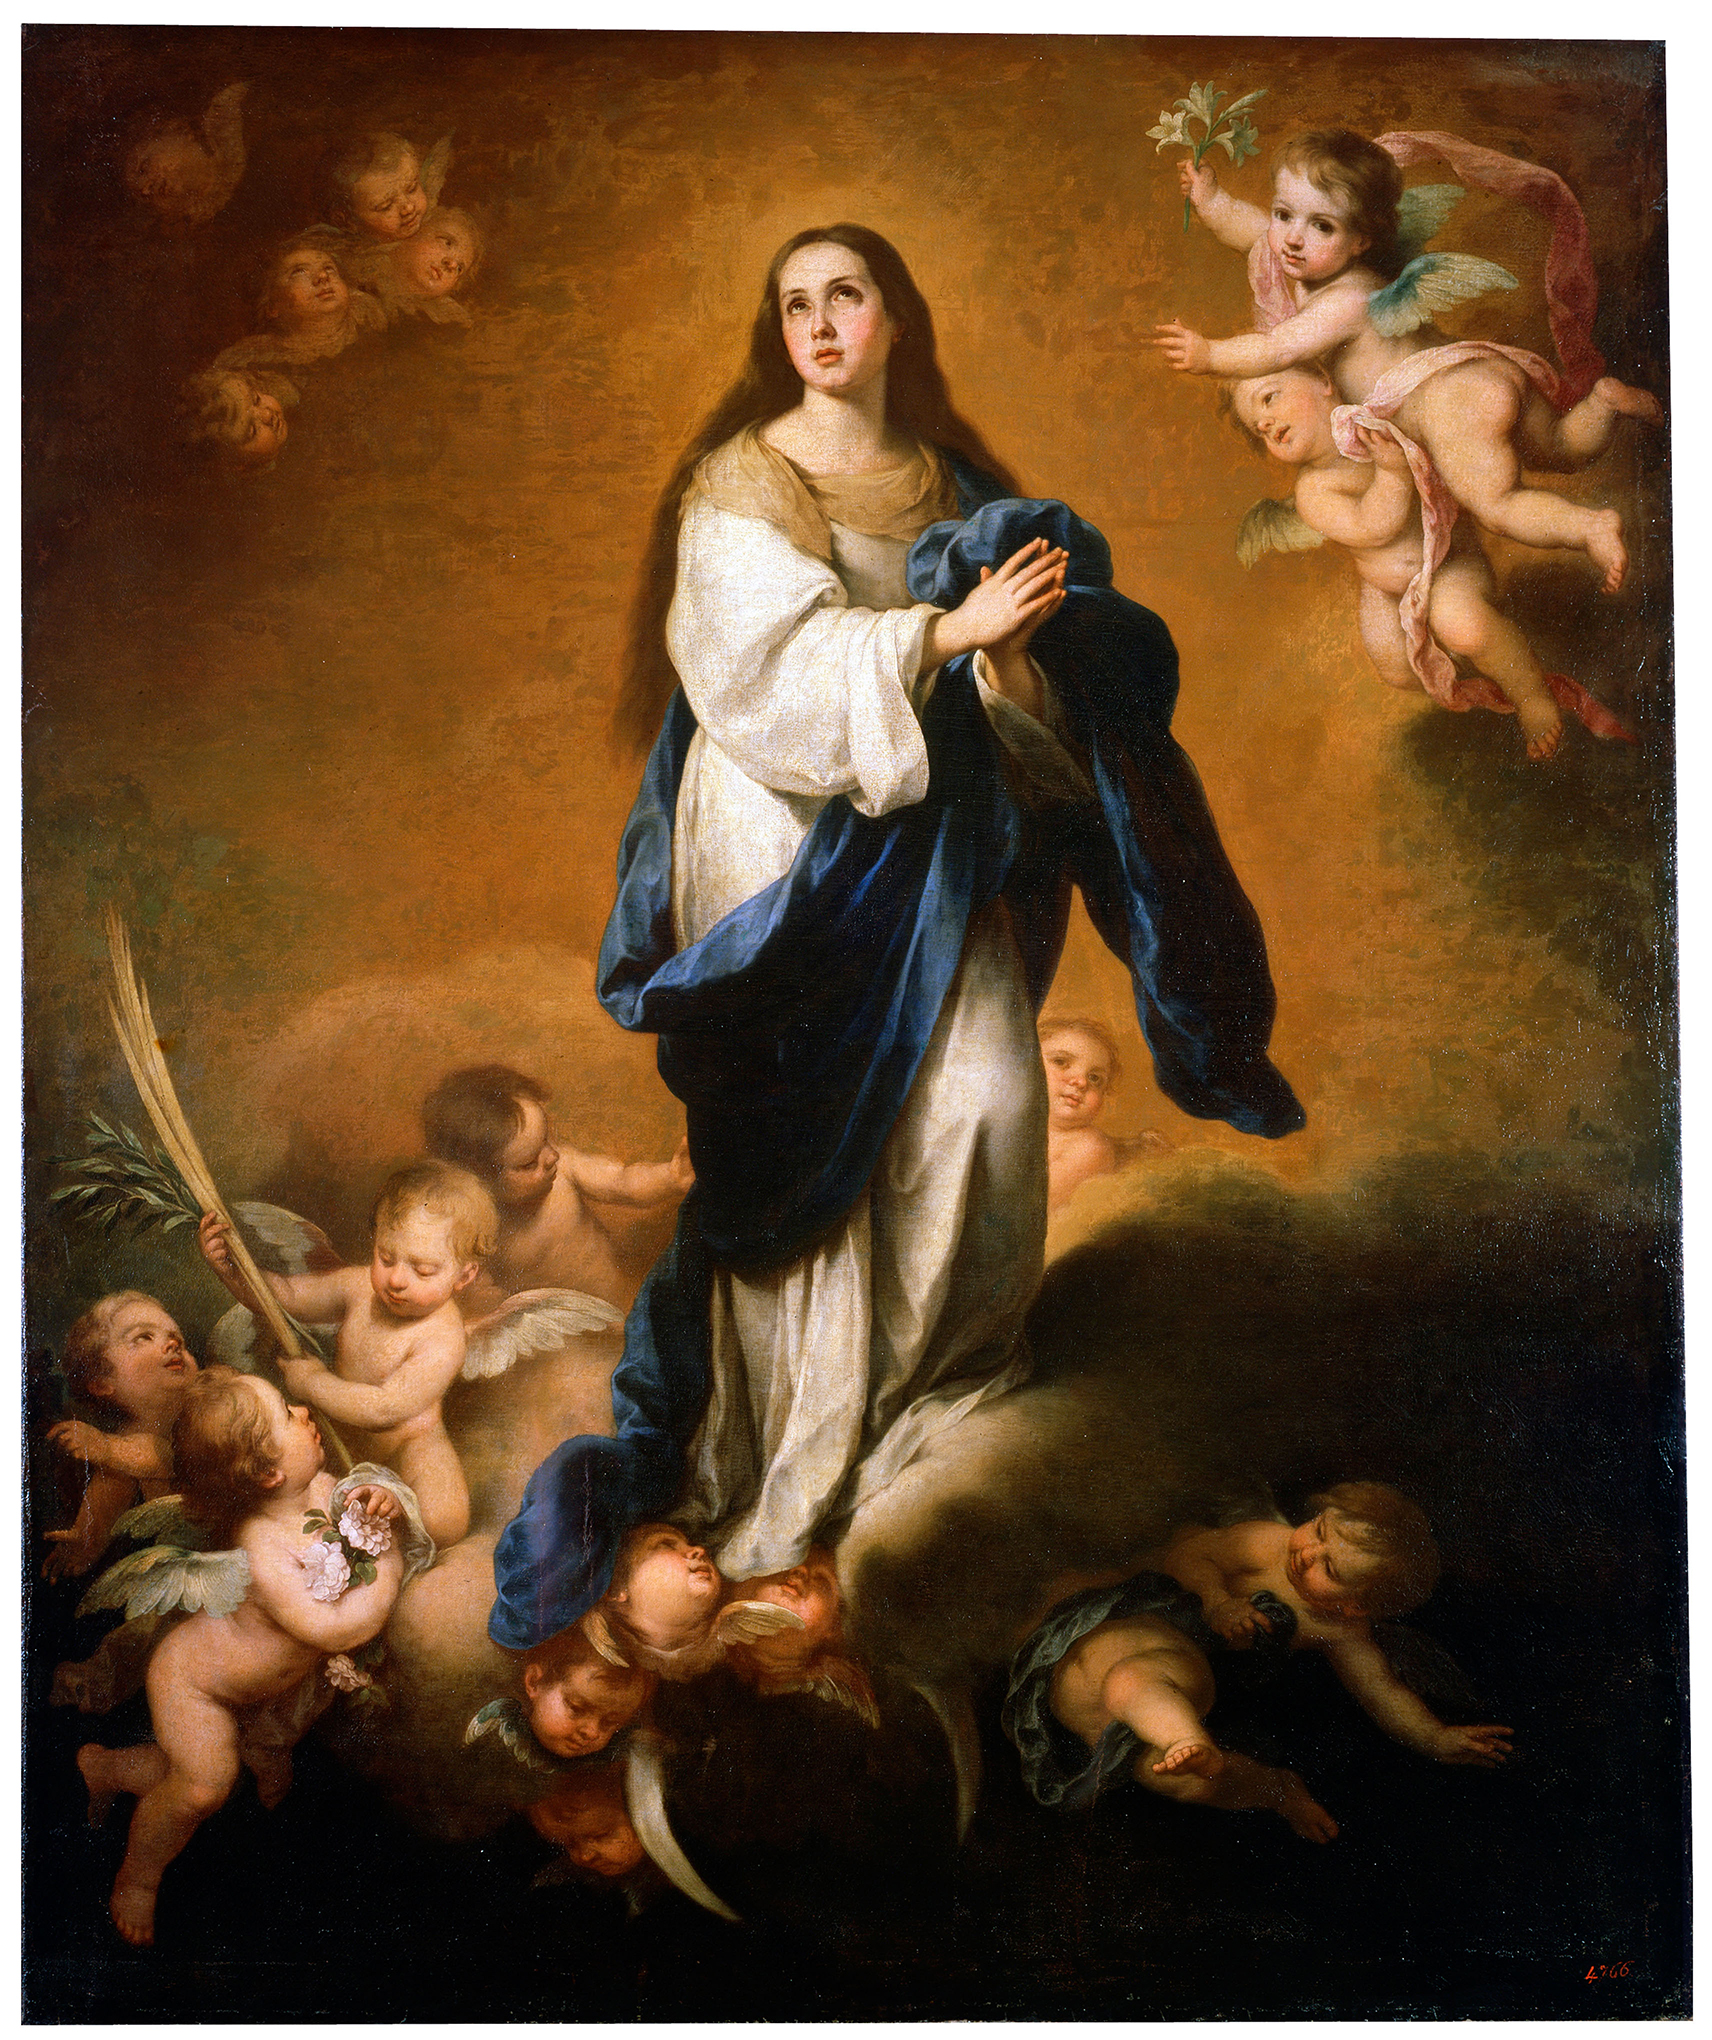
\includegraphics{foto-04.jpg}}\\
}
\author{Sergio}
\date{Valladolid (España), \monthyeardate\today}

\newcounter{joyful-counter}
\newcounter{sorrowful-counter}
\newcounter{glorious-counter}
\newcounter{lux-counter}

\setlength{\columnseprule}{0.5pt}
\colseprulecolor{red}
%\ensurevspace{50mm}

\begin{document}

\maketitle
%\afterpage{\blankpage}

\chapter*{Santo Rosario Meditado}

\begin{paracol}{2}
      \filacastellanolatin{oraciones/senal_cruz/castellano.tex}{oraciones/senal_cruz/latin.tex}
      \vspace{6mm}
      \filacastellanolatinsincro{oraciones/contricion/senor_mio_jesucristo.tex}{oraciones/contricion/confiteor/latin.tex}
      \vspace{2mm}
      \filacastellanolatinsincro{oraciones/versiculos/abre_senor_mis_labios/castellano.tex}{oraciones/versiculos/abre_senor_mis_labios/latin.tex}
      \vspace{2mm}
      \filacastellanolatinsincro{oraciones/versiculos/apresurate_snor/castellano.tex}{oraciones/versiculos/apresurate_snor/latin.tex}
      \vspace{2mm}
      \filacastellanolatinsincro{oraciones/gloria/castellano_separado.tex}{oraciones/gloria/latin_separado.tex}
      \vspace{2mm}
      \filacastellanolatinsincro{oraciones/versiculos/maria_madre/castellano.tex}{oraciones/versiculos/maria_madre/latin.tex}
\end{paracol}
\vspace{2mm}
\begin{center}
      \textcolor{red}{Decimos aquí las intenciones de este Rosario}
\end{center}
\vspace{2mm}
%%%%%%%%%%%%%%%%%%%%%%%%%%%%
% INICIO MISTERIOS GOZOSOS %
%%%%%%%%%%%%%%%%%%%%%%%%%%%%
\titulomisterio{Misterios Gozosos}{T: Lunes y jueves\\N: Lunes y sábados}\\[4mm]
%\vspace{4mm}
\titulomisterios{I La Anunciación de la Santísima Virgen María}{Lc 1, 27-33}
\vspace{2mm}
\primeraletragranderoja{Y}{}\space habiendo entrado a ella, dijo: <<Dios te salve, llena de gracia, el Señor es contigo, bendita tu entre las mujeres>>. Ella, al oír estas palabras, se turbó,
y discurría que podría ser esta salutación. Y le dijo el ángel: <<No temas, María, pues hallaste gracia a los ojos de Dios. He aquí que concebirás en tu seno y darás a luz un Hijo,
a quien darás por nombre Jesús. Este será grande, y será llamado Hijo del Altísimo, y le dará el Señor Dios el trono de David su padre, y reinará sobre la casa de Jacob etérnamente, 
y su reinado no tendrá fin>>.\\[-2mm]
\begin{paracol}{2}
    \filacastellanolatin{oraciones/padrenuestro/castellano_sencillo.tex}{oraciones/padrenuestro/latin_sencillo.tex}
    \vspace{2mm}
    \filacastellanolatinsincronota{\textcolor{red}{El avemaría se repite 10 veces}}{oraciones/avemaria/castellano_sencillo.tex}{oraciones/avemaria/latin_sencillo.tex}
    \vspace{6mm}
    \filacastellanolatinsincro{oraciones/gloria/castellano_separado.tex}{oraciones/gloria/latin_separado.tex}
    \vspace{2mm}
    \filacastellanolatinsincro{oraciones/versiculos/maria_madre/castellano.tex}{oraciones/versiculos/maria_madre/latin.tex}
\end{paracol}
\vspace{5mm}

\titulomisterios{II La Visitación de Nuestra Señora}{Lc 1, 39-45}
\vspace{2mm}
\primeraletragranderoja{P}{or}aquellos días, levantándose María, se dirigió presurosa a la montaña, a un ciudad de Judá, y entró en la casa de Zacarías y saludó a Isabel.
Y aconteció que, al oir Isabel la salutación de María, dió saltos de gozo el niño en su seno, y fue llena Isabel del Espíritu Santo, y levantó la voz con gran clamor y dijo:
Bendita tu entre las mujeres y bendito el fruto de tu vientre. {?`}Y de dónde a mí esto que venga la madre de mi Señor a mí? Porque he aquí que, como sonó la voz de tu salutación en mi oídos,
dió saltos de alborozo el niño en mi seno.\\[2mm]
\begin{center}
    Paternóster, diez Avemarías, Gloria

\end{center}

\begin{paracol}{2}
    \filacastellanolatin{oraciones/maria_madre/castellano_seguido.tex}{oraciones/maria_madre/latin_seguido.tex}
\end{paracol}
\vspace{5mm}

\titulomisterios{III La Natividad de Nuestro Señor Jesucristo}{Lc 2, 7-8.10-11}
\vspace{2mm}
\primeraletragranderojasola{Y}\space dió a luz su hijo primogénito, y le envolvió en pañales y le recostó en un pesebre, pues no había para ellos lugar en el mesón.
Y había unos pastores en aquella misma comarca, que pernoctaban al raso y velaban por turno para guardar su ganado, y un ángel del Señor se presentó ante ellos.
Y les dijo el Ángel: <<No temáis, pues he aquí que os traigo una buena nueva, que será de grande alegría para todo el pueblo: 
que os ha nacido hoy en la ciudad de David un Salvador, que es el Mesías, el Señor>>.\\[2mm]
\begin{center}
    Paternóster, diez Avemarías, Gloria

\end{center}

\begin{paracol}{2}
    \filacastellanolatin{oraciones/maria_madre/castellano_seguido.tex}{oraciones/maria_madre/latin_seguido.tex}
\end{paracol}
\vspace{5mm}

\titulomisterios{IV La Presentación del Niño Jesús en el Templo}{Lc 2, 22-24}
\vspace{2mm}
\primeraletragranderojasola{Y}\space cuando se les cumplieron los días de la purificación según la ley de Moisés, le subieron a Jerusalén para presentarle al Señor,
según está escrito en la Ley del Señor que <<todo primogénito del sexo masculino será consagrado al Señor>>, y para ofrecer como sacrificio,
según lo que se ordena en la Ley del Señor, <<un par de tórtolas o dos palominos>>.\\[2mm]
\begin{center}
    Paternóster, diez Avemarías, Gloria

\end{center}

\begin{paracol}{2}
    \filacastellanolatin{oraciones/maria_madre/castellano_seguido.tex}{oraciones/maria_madre/latin_seguido.tex}
\end{paracol}
\vspace{5mm}

\titulomisterios{V La pérdida y hallazgo del Niño Jesús en el Templo}{Lc 2, 46-48}
\vspace{2mm}
\primeraletragranderojasola{Y}\space no hallándole, se tornaron a Jerusalén para buscarle. Y sucedió que después de tres días le hallaron en el templo,
sentado en medio de los maestros, escuchándolos y haciéndoles preguntas; y se pasmaban todos los que le oían de su inteligencia y de sus respuestas.
Y sus padres, al verle, quedaron sorprendidos; y le dijo su madre: <<Hijo, {?`}por qué lo hiciste así con nosotros? Mira que tu padre y yo, llenos de aflicción, 
te andábamos buscando>>.\\[2mm]
{\begin{center}
    Paternóster, diez Avemarías, Gloria

\end{center}

\begin{paracol}{2}
    \filacastellanolatin{oraciones/maria_madre/castellano_seguido.tex}{oraciones/maria_madre/latin_seguido.tex}
\end{paracol}} Terminadas, nos vamos a la \cpageref{final-prayer} para las oraciones finales.\\[5mm]

%%%%%%%%%%%%%%%%%%%%%%%%%%%
% FINAL MISTERIOS GOZOSOS %
%%%%%%%%%%%%%%%%%%%%%%%%%%%
%\vspace{5mm}
%%%%%%%%%%%%%%%%%%%%%%%%%%%%%%
% INICIO MISTERIOS LUMINOSOS %
%%%%%%%%%%%%%%%%%%%%%%%%%%%%%%
\titulomisterio{Misterios Luminosos}{T: -\\N: Jueves }\\[4mm]
\titulomisterios{I El Bautismo del Señor en el Jordán}{Mc 1, 9-11}
%\vspace{2mm}
\primeraletragranderojasola{Y}\space aconteció por aquellos días que vino Jesús desde Nazaret de Galilea y fué bautizado en el Jordán por Juan el Bautista.
Y al punto subiendo del agua, vió rasgarse los cielos y venir sobre Él el Espíritu Santo como paloma; y una voz vino de los cielos: 
<<Tú eres mi Hijo amado, en Ti me agradé>>.\\[-2mm]
\begin{paracol}{2}
    \filacastellanolatin{oraciones/padrenuestro/castellano_sencillo.tex}{oraciones/padrenuestro/latin_sencillo.tex}
    \vspace{2mm}
    \filacastellanolatinsincronota{\textcolor{red}{El avemaría se repite 10 veces}}{oraciones/avemaria/castellano_sencillo.tex}{oraciones/avemaria/latin_sencillo.tex}
    \vspace{6mm}
    \filacastellanolatinsincro{oraciones/gloria/castellano_separado.tex}{oraciones/gloria/latin_separado.tex}
    \vspace{2mm}
    \filacastellanolatinsincro{oraciones/versiculos/maria_madre/castellano.tex}{oraciones/versiculos/maria_madre/latin.tex}
\end{paracol}
\vspace{5mm}

\titulomisterios{II Las Bodas de Caná}{Jn 2, 1-5}
\vspace{2mm}
\primeraletragranderoja{A}{l}tercer día hubo una boda en Caná de Galilea, y estaba allí la madre de Jesús. Fue invitado también Jesús con sus discípulos a la boda.
No tenían vino, porque el vino de la boda se había acabado. En esto dijo la madre de Jesús a este: No tiene vino. Díjole Jesús: Mujer,
{?`}qué nos va a mi y a ti? No es aún llegada mi hora. Dijo la madre a los servidores: Haced lo que Él os diga.\\[2mm]
\begin{center}
    Paternóster, diez Avemarías, Gloria

\end{center}

\begin{paracol}{2}
    \filacastellanolatin{oraciones/maria_madre/castellano_seguido.tex}{oraciones/maria_madre/latin_seguido.tex}
\end{paracol}
\vspace{5mm}

\titulomisterios{III El Anuncio del Reino de Dios}{Mc 1, 14-15.21-22}
\vspace{2mm}
\primeraletragranderoja{D}{espués}que Juan fue preso vino Jesús a Galilea predicando el Evangelio de Dios y diciendo: Cumplido es el tiempo, y el reino de Dios está cercano;
arrepentíos y creed en el Evangelio. Llegaron a Cafarnaúm, y luego, el día sábado, entrando en la sinagoga, enseñaba. Se maravillaban de su doctrina,
pues la enseñaba como quien tiene autoridad y no como los escribas.\\[2mm]
\begin{center}
    Paternóster, diez Avemarías, Gloria

\end{center}

\begin{paracol}{2}
    \filacastellanolatin{oraciones/maria_madre/castellano_seguido.tex}{oraciones/maria_madre/latin_seguido.tex}
\end{paracol}
\vspace{5mm}

\titulomisterios{IV La Transfiguración}{Mt 17, 1-3.5}
\vspace{2mm}
\primeraletragranderoja{S}{eis}días después tomó Jesús a Pedro, a Santiago y a Juan, su hermano, y los llevo aparte, a un monte alto. Y se transfiguró ante ellos;
brilló su rostro como el sol y sus vestidos se volvieron blancos como la luz. Aún estaba el hablando, cuando los cubrió una nube resplandeciente,
y salió de la nube una voz que decía: Este es mi Hijo amado, en quien tengo mi complacencia; escuchadle.\\[2mm]
\begin{center}
    Paternóster, diez Avemarías, Gloria

\end{center}

\begin{paracol}{2}
    \filacastellanolatin{oraciones/maria_madre/castellano_seguido.tex}{oraciones/maria_madre/latin_seguido.tex}
\end{paracol}
\vspace{5mm}

\titulomisterios{V La Institución de la Eucaristía}{Mt 26, 26-28}
\primeraletragranderoja{M}{ientras}comían, Jesús tomó pan, lo bendijo, lo partió y, dándoselo a los discípulos, dijo: Tomad y comed, éste es mi cuerpo. 
Y tomando un cáliz y dando gracias, se lo dió, diciendo: Bebed de él todos, que está es mi sangre del Nuevo Testamento, que será derramada por muchos 
para remisión de los pecados.\\[2mm]
{\begin{center}
    Paternóster, diez Avemarías, Gloria

\end{center}

\begin{paracol}{2}
    \filacastellanolatin{oraciones/maria_madre/castellano_seguido.tex}{oraciones/maria_madre/latin_seguido.tex}
\end{paracol}} Terminadas, nos vamos a la \cpageref{final-prayer} para las oraciones finales.\\[5mm]

%%%%%%%%%%%%%%%%%%%%%%%%%%%%%
% FINAÑ MISTERIOS LUMINOSOS %
%%%%%%%%%%%%%%%%%%%%%%%%%%%%%
%\vspace{5mm}
%%%%%%%%%%%%%%%%%%%%%%%%%%%%%%
% INICIO MISTERIOS DOLOROSOS %
%%%%%%%%%%%%%%%%%%%%%%%%%%%%%%
\titulomisterio{Misterios Dolorosos}{T: Martes y viernes\\N: Martes y viernes}\\[4mm]
\titulomisterios{I La oración en el Huerto de los Olivos}{Mc 14, 33-36}
\vspace{2mm}
\primeraletragranderoja{Y}{}\space lleva consigo a Pedro y a Santiago y a Juan, y comenzó a sentir espanto y abatimiento; y le dice: <<triste en gran manera está mi corazón hasta la muerte;
quedad aquí y velad>>. Y apartándose un poco, caía sobre tierra, y rogaba que, a ser posible, pasase el Él aquella hora, y decía: <<Abba, Padre, todas las cosas te son posibles:
traspasa de mi este cáliz; más no se haga lo que yo quiero, sino lo que tú quieres>>.\\[-2mm]
\begin{paracol}{2}
    \filacastellanolatin{oraciones/padrenuestro/castellano_sencillo.tex}{oraciones/padrenuestro/latin_sencillo.tex}
    \vspace{2mm}
    \filacastellanolatinsincronota{\textcolor{red}{El avemaría se repite 10 veces}}{oraciones/avemaria/castellano_sencillo.tex}{oraciones/avemaria/latin_sencillo.tex}
    \vspace{6mm}
    \filacastellanolatinsincro{oraciones/gloria/castellano_separado.tex}{oraciones/gloria/latin_separado.tex}
    \vspace{2mm}
    \filacastellanolatinsincro{oraciones/versiculos/maria_madre/castellano.tex}{oraciones/versiculos/maria_madre/latin.tex}
\end{paracol}
\vspace{5mm}

\titulomisterios{II La Flagelación de Nuestro Señor Jesucristo}{Jn 18,38-40; 19, 1}
\vspace{2mm}
\primeraletragranderoja{\guillemotleft Y}{o}no hallo en Él delito alguno. Es costumbre vuestra que yo os suelte un preso por la Pascua: {?`}queréis, 
pues, que os suelte al rey de los Judíos?\guillemotright. Gritaron, pues, de nuevo, diciendo: <<No, a ése, sino a Barrabás>>. 
Era este Barrabás un salteador. Entonces, pues, tomó Pilato a Jesús y le azotó.\\[2mm]
\begin{center}
    Paternóster, diez Avemarías, Gloria

\end{center}

\begin{paracol}{2}
    \filacastellanolatin{oraciones/maria_madre/castellano_seguido.tex}{oraciones/maria_madre/latin_seguido.tex}
\end{paracol}
\vspace{5mm}

\titulomisterios{III La Coronación de espinas de Nuestro Señor Jesucristo}{Mt 27, 27-30}
\vspace{2mm}
\primeraletragranderoja{E}{ntonces}los soldados del gobernador, tomando a Jesús y conduciéndole al pretorio, reunieron en torno a Él toda la cohorte. 
Y habiéndole quitado sus vestidos, le envolvieron en una clámide de grana, y trenzando una corona de espinas, la pusieron sobre su cabeza, 
y una caña en su mano derecha; y doblando la rodilla delante de Él, le mofaban, diciendo: <<Salud, Rey de los judíos>>. Y escupiendo en Él, 
tomaron la caña y le daban golpes en la cabeza.\\[2mm]
\begin{center}
    Paternóster, diez Avemarías, Gloria

\end{center}

\begin{paracol}{2}
    \filacastellanolatin{oraciones/maria_madre/castellano_seguido.tex}{oraciones/maria_madre/latin_seguido.tex}
\end{paracol}
\vspace{5mm}

\titulomisterios{IV El Señor con la cruz a cuestas}{Jn 19, 16-17; Lc 23, 26}
\vspace{2mm}
\primeraletragranderoja{E}{ntonces,}pues, se le entregó para que fuera crucificando. Se apoderaron, pues, de Jesús, y llevando a cuestas su cruz, 
salió hacia el lugar llamado el Cráneo, que en hebreo se dice Gólgota. Y como le hubieron sacado, echaron mano de un tal Simón de Cirene que venía del campo, 
le pusieron en hombros la cruz para que la llevase detrás de Jesús.\\[2mm]
\begin{center}
    Paternóster, diez Avemarías, Gloria

\end{center}

\begin{paracol}{2}
    \filacastellanolatin{oraciones/maria_madre/castellano_seguido.tex}{oraciones/maria_madre/latin_seguido.tex}
\end{paracol}
\vspace{5mm}

\titulomisterios{V Crucifixión y Muerte del Redentor}{Lc 23, 33-34; Jn 19, 19.25-27;\\Lc 23, 44-46}
\vspace{2mm}
\primeraletragranderoja{C}{uando}llegaron al lugar llamado Calvario, le crucificaron allí, y a los dos malhechores, uno a la derecha y otro a la izquierda. 
Jesús decía: Padre, perdónalos, porque no saben los que hacen. Dividiendo sus vestidos, echaron suertes sobre ellos. Escribió Pilato un título y lo puso sobre la cruz;
estaba escrito: \textit{Jesús Nazareno, Rey de los judíos}. Estaba junto a la cruz de Jesús su Madre y la hermana de su Madre, María la debajo Cleofás y María Magdalena.
Jesús, viendo a su Madre y al discípulo a quien amaba, que estaba allí, dijo a la Madre: Mujer, he ahí a tu hijo. Luego dijo al discípulo: He ahí a tu Madre.
Y desde aquella hora el discípulo la recibió en su casa. Era ya como la hora de sexta, y las tinieblas cubrieron toda la tierra hasta la hora de nona,
obscurecióse el sol y el velo del templo se rasgó por medio. Jesús, dando una gran voz, dijo: Padre, en tus manos entrego mi espíritu; y diciendo esto expiró.\\[2mm]
{\begin{center}
    Paternóster, diez Avemarías, Gloria

\end{center}

\begin{paracol}{2}
    \filacastellanolatin{oraciones/maria_madre/castellano_seguido.tex}{oraciones/maria_madre/latin_seguido.tex}
\end{paracol}} Terminadas, nos vamos a la \cpageref{final-prayer} para las oraciones finales.\\[5mm]

%%%%%%%%%%%%%%%%%%%%%%%%%%%%%
% FINAL MISTERIOS DOLOROSOS %
%%%%%%%%%%%%%%%%%%%%%%%%%%%%%
%\vspace{5mm}
%%%%%%%%%%%%%%%%%%%%%%%%%%%%%%
% INICIO MISTERIOS GLORIOSOS %
%%%%%%%%%%%%%%%%%%%%%%%%%%%%%%
\titulomisterio{Misterio Gloriosos}{T: Miércoles, sábados y domingos\\N: Miércoles y domingos}\\[4mm]
\titulomisterios{I La Resurrección del Señor}{Mt 28, 1-3.5-7}
\vspace{2mm}
\primeraletragranderoja{P}{asado}el sábado, ya para amanecer el día primero de la semana, vino María Magdalena con la otra María al sepulcro. Y sobrevino un gran terremoto,
pues un ángel del Señor bajó del cielo y acercándose removió la piedra del sepulcro y se sentó sobre ella. Era su aspecto como el relámpago, y su vestidura blanca como la nueve.
El ángel, dirigiéndose a las mujeres, dijo: No temáis vosotras, pues sé que buscáis a Jesús el crucificado. No está aquí; ha resucitado, según lo había dicho.
Venid y ved el sitio donde fue puesto. Id luego y decid a sus discípulos que ha resucitado de entre los muertos y que os precede a Galilea; allí le veréis.
Es lo que tenía que deciros.\\[-2mm]
\begin{paracol}{2}
    \filacastellanolatin{oraciones/padrenuestro/castellano_sencillo.tex}{oraciones/padrenuestro/latin_sencillo.tex}
    \vspace{2mm}
    \filacastellanolatinsincronota{\textcolor{red}{El avemaría se repite 10 veces}}{oraciones/avemaria/castellano_sencillo.tex}{oraciones/avemaria/latin_sencillo.tex}
    \vspace{6mm}
    \filacastellanolatinsincro{oraciones/gloria/castellano_separado.tex}{oraciones/gloria/latin_separado.tex}
    \vspace{2mm}
    \filacastellanolatinsincro{oraciones/versiculos/maria_madre/castellano.tex}{oraciones/versiculos/maria_madre/latin.tex}
\end{paracol}
\vspace{5mm}

\titulomisterios{II Las Ascensión Jesucristo a los cielos}{Lc 24, 50; Mc 16, 15-16.19-20}
\vspace{2mm}
\primeraletragranderoja{L}{os}llevó hasta cerca de Betania, y levantando sus manos les bendijo. Y les dijo: Id al mundo entero y predicad el Evangelio a toda la creación.
El que creyere y fuere bautizado, se salvará, mas el que no creyere, será condenado. Con esto el Señor Jesús, después de hablarles, fue elevado al cielo y se sentó a la diestra de Dios.
Y ellos, partiéndose de allí, predicaron por todas partes, cooperando el Señor y confirmando la palabra con las señales que la acompañaban.\\[2mm]
\begin{center}
    Paternóster, diez Avemarías, Gloria

\end{center}

\begin{paracol}{2}
    \filacastellanolatin{oraciones/maria_madre/castellano_seguido.tex}{oraciones/maria_madre/latin_seguido.tex}
\end{paracol}
\vspace{5mm}

\titulomisterios{III La Venida del Espíritu Santo sobre los Apóstoles}{Jn 14, 26; Hch. 2, 1-4}
\vspace{2mm}
\primeraletragranderoja{M}{as}el Paráclito, el Espíritu Santo, que enviará el Padre en mi nombre, Él os enseñará todas las cosas y os recordará todas las cosas que os dije yo.
Y al cumplirse el día de Pentecostés, estaban todos juntos en el mismo lugar. Y se produjo de súbito desde el cielo un estruendo como de viento que soplaba vehementemente,
y llenó toda la casa donde se hallaban sentados. Y vieron aparecer lenguas como de fuego, que, repartiéndose, se posaban sobre cada uno de ellos.\\[2mm]
\begin{center}
    Paternóster, diez Avemarías, Gloria

\end{center}

\begin{paracol}{2}
    \filacastellanolatin{oraciones/maria_madre/castellano_seguido.tex}{oraciones/maria_madre/latin_seguido.tex}
\end{paracol}
\vspace{5mm}

\titulomisterios{IV La Asunción de María Santísima a los cielos}{Lc 1, 46-49; Ap 11, 19}
\vspace{2mm}
\primeraletragranderoja{M}{i}alma magnifica al Señor y exulta de júbilo mi espíritu al Señor, mi Salvador, porque ha mirado la humildad de su sierva;
por eso todas las generaciones me llamarán bienaventurada, porque ha hecho en mi maravillas el Poderoso, cuyo nombre es santo. Y se abrió el templo de Dios, que está en el cielo,
y fué vista el arca de la alianza en el templo, y se produjeron relámpagos, y voces, y truenos, y temblor de tierra, y fuerte granizada.\\[2mm]
\begin{center}
    Paternóster, diez Avemarías, Gloria

\end{center}

\begin{paracol}{2}
    \filacastellanolatin{oraciones/maria_madre/castellano_seguido.tex}{oraciones/maria_madre/latin_seguido.tex}
\end{paracol}
\vspace{5mm}

\titulomisterios{V La Coronación de la Santísima Virgen María}{Cant 6,10; Ap 12, 1; 18, 16;\\Sal 44, 10}
\vspace{2mm}
\primeraletragranderoja{{?`}Q}{uién}es esa que aparece resplandeciente como la aurora, hermosa cual luna, deslumbradora como el sol, imponente como batallones?.
Y una gran señal fué vista en el cielo: una Mujer vestida del sol, y la luna debajo de sus  pies, y sobre su cabeza una corona de doce estrellas.
Tiene Él escrito en su vestido y en su manto Rey de reyes y Señor de los que dominan. Está la Reina a su derecha, adornada con oro finísimo.\\[2mm]
\begin{center}
    Paternóster, diez Avemarías, Gloria

\end{center}

\begin{paracol}{2}
    \filacastellanolatin{oraciones/maria_madre/castellano_seguido.tex}{oraciones/maria_madre/latin_seguido.tex}
\end{paracol}
\vspace{5mm}

%%%%%%%%%%%%%%%%%%%%%%%%%%%%%
% FINAL MISTERIOS GLORIOSOS %
%%%%%%%%%%%%%%%%%%%%%%%%%%%%%
%%%%%%%%%%%%%%%%%%%%%%%%%%%%%%%%
% ORACIONES FINALES Y LETANIAS %
%%%%%%%%%%%%%%%%%%%%%%%%%%%%%%%%
\label{final-prayer}
\begin{center}
      \textcolor{red}{Terminados los misterios podemos rezar}
\end{center}

\begin{paracol}{2}
      \filacastellanolatin{oraciones/avemaria/hija/castellano.tex}{oraciones/avemaria/hija/latin.tex}
      \vspace{6mm}
      \filacastellanolatinsincro{oraciones/avemaria/madre/castellano.tex}{oraciones/avemaria/madre/latin.tex}
      \vspace{6mm}
      \filacastellanolatinsincro{oraciones/avemaria/esposa/castellano.tex}{oraciones/avemaria/esposa/latin.tex}
      \vspace{6mm}
      \filacastellanolatinsincro{oraciones/avemaria/sagrario/castellano.tex}{oraciones/avemaria/sagrario/latin.tex}
\end{paracol}
\vspace{3mm}
\begin{center}
      \textcolor{red}{Letanías de Nuestra Señora}
\end{center}

\begin{paracol}{2}
      \filacastellanolatin{oraciones/letanias/castellano.tex}{oraciones/letanias/latin.tex}
      \vspace{2mm}
      \filacastellanolatinsincro{oraciones/bajo_tu_amparo/castellano.tex}{oraciones/bajo_tu_amparo/latin.tex}
\end{paracol}
\vspace{4mm}
\textopequenorojo{Desde la Purificación hasta Sábado Santo y desde la Santísima Trinidad hasta el I Domingo de Adviento:}
\begin{paracol}{2}
      \filacastellanolatin{oraciones/versiculos/salve/castellano.tex}{oraciones/versiculos/salve/latin.tex}
      \vspace{6mm}
      \filacastellanolatinsincro{oraciones/antifonas_bvm/01_septuagesima_cuaresma_postpentecostes/castellano.tex}{oraciones/antifonas_bvm/01_septuagesima_cuaresma_postpentecostes/latin.tex}
\end{paracol}
\vspace{4mm}
\textopequenorojo{Desde el I Domingo de Adviento hasta Navidad:}
\begin{paracol}{2}
      \filacastellanolatin{oraciones/angelus/castellano_00.tex}{oraciones/angelus/latin_00.tex}
      \vspace{2mm}
      \filacastellanolatinsincro{oraciones/antifonas_bvm/02_adviento/castellano.tex}{oraciones/antifonas_bvm/02_adviento/latin.tex}
\end{paracol}
\vspace{4mm}
\textopequenorojo{Desde Navidad hasta la Purificación:}
\begin{paracol}{2}
      \filacastellanolatin{oraciones/antifonas_bvm/03_navidad/castellano_00.tex}{oraciones/antifonas_bvm/03_navidad/latin_00.tex}
      \vspace{2mm}
      \filacastellanolatinsincro{oraciones/antifonas_bvm/03_navidad/castellano_01.tex}{oraciones/antifonas_bvm/03_navidad/latin_01.tex}
\end{paracol}
\newpage
\textopequenorojo{Desde Domingo de Resurrección hasta la Santísima Trinidad:}
\begin{paracol}{2}
      \filacastellanolatin{oraciones/regina_coelis/castellano_00.tex}{oraciones/regina_coelis/latin_00.tex}
      \vspace{2mm}
      \filacastellanolatinsincro{oraciones/antifonas_bvm/04_pascua/castellano.tex}{oraciones/antifonas_bvm/04_pascua/latin.tex}
\end{paracol}
\vspace{4mm}
\textopequenorojo{Rezamos ahora por el Santo Padre, nuestro Obispo y los fieles difuntos:}
\begin{paracol}{2}
      \filacastellanolatin{oraciones/versiculos/el_senor_este/castellano.tex}{oraciones/versiculos/el_senor_este/latin.tex}
      \vspace{1mm}
      \filacastellanolatinsincro{oraciones/por_el_papa/castellano.tex}{oraciones/por_el_papa/latin.tex}
      \vspace{1mm}
      \filacastellanolatinsincro{oraciones/padrenuestro/castellano_sencillo.tex}{oraciones/padrenuestro/latin_sencillo.tex}
      \vspace{1mm}
      \filacastellanolatinsincro{oraciones/avemaria/castellano_sencillo.tex}{oraciones/avemaria/latin_sencillo.tex}
      \vspace{5.5mm}
      \filacastellanolatinsincro{oraciones/gloria/castellano_seguido.tex}{oraciones/gloria/latin_seguido.tex}
      \vspace{2mm}
      \filacastellanolatinsincro{oraciones/por_el_obispo/castellano.tex}{oraciones/por_el_obispo/latin.tex}
      \vspace{6mm}
      \begin{leftcolumn*}
            Padre nuestro, Ave María y Gloria.
      \end{leftcolumn*}
      \begin{otherlanguage}{latin}
            \begin{rightcolumn}
                  Pater noster, Ave María et Glória.
            \end{rightcolumn}
      \end{otherlanguage}
      \vspace{2mm}
      \filacastellanolatinsincro{oraciones/por_los_fieles_difuntos/castellano_00.tex}{oraciones/por_los_fieles_difuntos/latin_00.tex}
      \vspace{1mm}
      \begin{leftcolumn*}
            Padre nuestro y Ave María.
      \end{leftcolumn*}
      \begin{otherlanguage}{latin}
            \begin{rightcolumn}
                  Pater noster et Ave María.
            \end{rightcolumn}
      \end{otherlanguage}
      \vspace{1mm}
      \filacastellanolatinsincro{oraciones/por_los_fieles_difuntos/castellano_01.tex}{oraciones/por_los_fieles_difuntos/latin_01.tex}
      \vspace{2mm}
      \filacastellanolatinsincro{oraciones/versiculos/escucha_senor/castellano.tex}{oraciones/versiculos/escucha_senor/latin.tex}
\end{paracol}
\vspace{4mm}
Una Salve al Inmaculado Corazón de María:
\begin{paracol}{2}
      \filacastellanolatin{oraciones/salve/castellano.tex}{oraciones/salve/latin.tex}
\end{paracol}
\newpage
Un Credo al Sagrado Corazón de Jesús:
\begin{paracol}{2}
      \filacastellanolatin{oraciones/credo/apostoles_castellano.tex}{oraciones/credo/apostoles_latin.tex}
      \vspace{6mm}
      \filacastellanolatinsincro{oraciones/san_jose/castellano.tex}{oraciones/san_jose/latin.tex}
      \vspace{11mm}
      \filacastellanolatinsincro{oraciones/san_miguel/castellano.tex}{oraciones/san_miguel/latin.tex}
\end{paracol}
\vspace{2mm}
\textopequenorojo{Se repite tres veces}
\begin{paracol}{2}
      \filacastellanolatin{oraciones/versiculos/corazon_jesus/castellano.tex}{oraciones/versiculos/corazon_jesus/latin.tex}
      \vspace{2mm}
      \filacastellanolatinsincro{oraciones/versiculos/avemaria_purisima/castellano.tex}{oraciones/versiculos/avemaria_purisima/latin.tex}
      \vspace{2mm}
      \filacastellanolatinsincro{oraciones/senal_cruz/castellano.tex}{oraciones/senal_cruz/latin.tex}
\end{paracol}
%%%%%%%%%%%%%%%%%%%%%%%%%%%%%%%%
% ORACIONES FINALES Y LETANIAS %
%%%%%%%%%%%%%%%%%%%%%%%%%%%%%%%%
%%%%%%%%%%%%%%%%%%%%%%%%%%%
% ANGELUS Y REGINA COELIS %
%%%%%%%%%%%%%%%%%%%%%%%%%%%
\chapter*{Ángelus y Regina C{\oe}li}

\begin{paracol}{2}

      \filacastellanolatinsincronota{\section*{Ángelus}}
            {oraciones/angelus/castellano_00.tex}
            {oraciones/angelus/latin_00.tex}
      \vspace{1mm}
      \filacastellanolatinsincro{oraciones/avemaria/castellano_sencillo.tex}{oraciones/avemaria/latin_sencillo.tex}
      \vspace{6mm}
      \filacastellanolatinsincro{oraciones/angelus/castellano_01.tex}{oraciones/angelus/latin_01.tex}
      \vspace{1mm}
      \filacastellanolatinsincro{oraciones/avemaria/castellano_inicio.tex}{oraciones/avemaria/latin_inicio.tex}
      \vspace{1mm}
      \filacastellanolatinsincro{oraciones/angelus/castellano_02.tex}{oraciones/angelus/latin_02.tex}
      \vspace{1mm}
      \filacastellanolatinsincro{oraciones/avemaria/castellano_inicio.tex}{oraciones/avemaria/latin_inicio.tex}
      \vspace{1mm}
      \filacastellanolatinsincro{oraciones/versiculos/salve/castellano.tex}{oraciones/versiculos/salve/latin.tex}
      \vspace{5mm}
      \filacastellanolatinsincro{oraciones/angelus/castellano_03.tex}{oraciones/angelus/latin_03.tex}

      \filacastellanolatinsincronota{\section*{Regina C{\oe}li L{\ae}táre (Tiempo Pascual)}}
            {oraciones/regina_coelis/castellano_00.tex}
            {oraciones/regina_coelis/latin_00.tex}
      \vspace{2mm}
      \filacastellanolatinsincro{oraciones/regina_coelis/castellano_01.tex}{oraciones/regina_coelis/latin_01.tex}

\end{paracol}
%%%%%%%%%%%%%%%%%%%%%%%%%%%
% ANGELUS Y REGINA COELIS %
%%%%%%%%%%%%%%%%%%%%%%%%%%%
\end{document}